\documentclass[12pt,reqno]{article} %\bibliographystyle{jasanum}

\usepackage[utf8x]{inputenc}
\usepackage{amsmath,amsfonts,amssymb,amscd,amsthm,xspace}
\usepackage{subfigure}
\usepackage{graphicx}
\usepackage{hyperref}
\usepackage{capt-of}
\renewcommand\refname{Bibliography}
\usepackage{setspace}
%\usepackage{lipsum}
\usepackage{natbib}
\bibliographystyle{jasaauthyear}
\usepackage{parskip}
% smaller margins:
\usepackage{fullpage}
\usepackage{tabu}
\usepackage{array}


%\renewcommand{\baselinestretch}{2}
% \renewcommand{\section}[1]{\medskip \addtocounter{section}{1}\raggedright 
%     \textbf{\Roman{section}. \ #1}\medskip \setcounter{subsection}{0}
%    \setlength{\parindent}{5ex}
% }
% \renewcommand{\subsection}[1]{\medskip \addtocounter{subsection}{1}\raggedright
%    \textbf{\Alph{subsection}. \ #1} \medskip \setcounter{subsubsection}{0}  
%    \setlength{\parindent}{5ex}
% }



\renewcommand{\thesection}{\Roman{section}}
\renewcommand{\thesubsection}{\thesection.\Alph{subsection}}


 \renewcommand{\bibsection}{\medskip \raggedright  \textbf{REFERENCES}
    \medskip}

\renewcommand{\bibnumfmt}[1]{\textbf{{#1}.}\ \ }


 \setlength{\parindent}{5ex}
 \setlength{\paperwidth}{8.5in}
 \setlength{\textwidth}{6.5in}
 \setlength{\oddsidemargin}{0in}
 \setlength{\evensidemargin}{0in}

   


%\newcommand{\cp}{   \ensuremath{v_{\text{P}}}}
%\newcommand{\vp}{   \ensuremath{v_{\text{x}}}}
%\newcommand{\vs}{   \ensuremath{v_{\text{S}}}}
%\newcommand{\vsh}{  \ensuremath{v_{\text{y}}}}
%\newcommand{\vsv}{  \ensuremath{v_{\text{z}}}}
%\newcommand{\MPa}{  \ensuremath{\text{MPa}}}
%\newcommand{\ms}{   \ensuremath{ \frac{\text{m}}{\text{s}}}}
%\newcommand{\kms}{  \ensuremath{ \frac{\text{km}}{\text{s}}}}
%\newcommand{\mh}{   \ensuremath{ \frac{\text{m}}{\text{h}}}}
%\newcommand{\kHz}{  \ensuremath{\text{kHz}}}
 
\begin{document}
% 

%\title[Structural monitoring with traffic recordings ]{Structural monitoring of a highway bridge using passive noise recordings from street traffic }
\title{An Event Database for Rotational Seismology}

\author{Johannes Salvermoser, Bryant Chow, C\'{e}line Hadziioannou, Sarah Hable, Lion Krischer, Catalina-M. Ramos-Domke, Joachim Wassermann, Ulrich Schreiber, Andre Gebauer, and Heiner Igel}

%\email[]{hadzii@geophysik.uni-muenchen.de}
%\homepage[]{Your web page}
%\thanks{}
%\altaffiliation{}
%\affiliation{Department for Earth- and Environmental Sciences\\ Ludwig-Maximilians-University\\ Theresienstrasse 41, 80333 Munich
 %Author's affiliation
%}
% 
% 
% 
%\date{\today}
% 

\begin{center}

\textbf{An Event Database for Rotational Seismology}

\vspace{6em}
Johannes Salvermoser\footnote{email: jsalvermoser@geophysik.uni-muenchen.de}, Bryant Chow, C\'{e}line Hadziioannou, Sarah Hable, Lion Krischer, Catalina-M. Ramos-Domke, Joachim Wassermann, Ulrich Schreiber, Andre Gebauer, and Heiner Igel
\vspace{3em}

Department for Earth- and Environmental Sciences\\ Ludwig-Maximilians-University\\ Theresienstrasse 41, 80333 Munich


%Pacs: 43.40.Le, 43.40.Ph, 43.20.Jr, 43.20.Fn

\end{center}

\begin{abstract}
Structural damage on bridges presents a hazard to public safety and can lead to fatalities. This article contributes to the development of an alternative monitoring system for civil structures, based on passive measurements of seismic elastic waves. Cross-correlations of traffic noise recorded at geophone receiver pairs were found to be sufficiently stable for comparison and sensitive to velocity changes in the medium. As such velocity variations could be caused by damage, their detection would be valuable in structural health monitoring systems.

\end{abstract}
%\newpage
% 
%\pacs{%
%43.40.Le, 43.40.Ph, 43.20.Jr, 43.20.Fn
%}
% 
%\keywords{Non-Destructive Testing \sep Concrete Bridge \sep Passive Image Interferometry \sep Cross-correlation \sep Structural Health Monitoring \sep Coda Wave Interferometry}
%\maketitle must follow title, authors, abstract, \pacs, and \keywords
%\maketitle
% 
%%%%%%%%%%%%%%%%%%%%%%%%%%%%%%%%%%%%%%%%%%%%%%%%%%%%%%%%%%%%%%%%%%%%%%%%%%%%%%
%%%%%%%%% SECTION INTRODUCTION
%%%%%%%%%%%%%%%%%%%%%%%%%%%%%%%%%%%%%%%%%%%%%%%%%%%%%%%%%%%%%%%%%%%%%%%%%%%%%%
% 
\section{Introduction}
Since the beginning of the 20th century, seismology has been dominated by only one type of observation: translational ground motions (usually measured as three orthogonal components: N-S, E-W, vertical). In the past two decades, due to the emerging ring laser gyroscope development and its calibration to high sensitivities \citep{Stedman1995,Stedman1997,Schreiber2003, Schreiber2004} for geodetic applications, rotational ground motions have become available as a new observable in seismology. \cite{AkiRichards2002} have proposed that the additional three components of rotational ground motion in a single measurement point will allow us to completely reconstruct local ground motion.\\ 
In this regard, \cite{Igel2005} and \cite{Kurrle2010} found that from amplitude ratios from this single point measurement, it is possible to retrieve dispersion curves of Love waves generated by (teleseismic) earthquakes.\\
Another aspect that was only feasible with seismic array measurements (e.g. beam-forming) before is the estimation of the event source direction. \cite{Igel2007} showed a straight-forward approach to infer the source direction (=backazimuth) from  collocated broadband seismometer and ring laser recordings using a cross-correlation grid search.

This project was initiated for two reasons:\\ 
$[1]$ the first main goal is to make processed ring laser data publicly available in order to promote its usage and significance for seismological applications. In this context, we built up an event database containing processed event plots and separate metadata files.\\
$[2]$ The second goal is to show how ring laser waveforms (here vertical component rotation rates from Wettzell “G-Ring”) can be accessed and processed. For that purpose, we provide tutorials in terms of open source ObsPy \citep{Megies2011,Krischer2015} based Jupyter Notebooks \citep{Perez2007} which graphically and interactively present the basic processing - as used for the database - while providing helpful background information.
\\
Currently, as mentioned before, we process data provided by a single station, the Wettzell Geodetic Observatory in S-E Germany. The 4 x 4 m ring laser “G-Ring”, located there, measures the Sagnac-interference at very high precision, yielding a sensitivity to rotations around the vertical axis that is high enough to record even teleseismic events at reasonable signal-to-noise ratio.
Translational ground motions are measured parallel to the rotations using a collocated STRECKEISEN STS-2 broadband seismometer.
\\
%This study aims towards the development of a passive time-domain technique for monitoring of civil structures. It applies the seismological method of passive image interferometry to small scales. To that end, 27 geophones were installed in the girder of a 229~m long highway bridge, and have been recording the vertical motion of the bottom slab continuously (sec. \ref{sec:measurement_setup}). The main observation is that the recorded signal is dominated by traffic induced noise and that the strongest peaks come from cars crossing the extension gap at either end of the bridge (sec. \ref{sec:measurement_signal}). Section \ref{sec:processing} explains how that signal can be used for passive image interferometry. The results, presented in sec. \ref{sec:results} show that the temperature signature on the elastic wave velocities can be measured efficiently with PII using traffic noise. This is promising, as it means the method of PII could be applied to a range of structures where strong cultural noise sources, like car traffic, are available. Our results have been tested for biases caused by temperature sensitivity of the sensors in sec. \ref{sec:discussion_reliability} and compared with prior studies using active measurements on bridges and in the laboratory in sec. \ref{sec:discussion_comparison}. The discussion concludes with an examination of the relation between temperature and velocity changes (sec. \ref{sec:discussion_temperature}).\\
% 
%%%%%%%%%%%%%%%%%%%%%%%%%%%%%%%%%%%%%%%%%%%%%%%%%%%%%%%%%%%%%%%%%%%%%%%%%%%%%%
%%%%%%%%% SECTION METHOD
%%%%%%%%%%%%%%%%%%%%%%%%%%%%%%%%%%%%%%%%%%%%%%%%%%%%%%%%%%%%%%%%%%%%%%%%%%%%%%
% 
\section{Website}
\label{sec:website}

The website provides the caller/visitor with a graphical user interface of the database and several additional information and links to topic-related projects.
Upon defining filter parameters (time period, magnitude, latitude/longitude), the user gets a map representation of the specified available event catalog.  In the zoomable world map, the earthquake events markers are sized and dyed according to the earthquake’s moment magnitude and source depth, respectively. This is intended to help finding the desired event more quickly.
By clicking on the event markers, the user opens a popup menu yielding a short description of the event by means of source time, magnitude and depth. The popup also contains links to a couple of images for the processed waveform data of rotational and translational ground motions:

\begin{itemize}
	\item Event information
	\item Waveform comparison
	\item Parameter estimation (Love wave phase velocity, backazimuth)
	\item P-coda analysis
\end{itemize}

Finally, it comprises a metadata parameter file in the easily (machine-) readable json-dictionary format. This dictionary contains all event and data fetching information and most importantly processed parameters such as  peak values (displacement, acceleration, rotation rate, correlation), signal-to-noise ratios, mean phase velocities (+ STDs), estimated and theoretical backazimuth.
\begin{figure*}[!htp]
\centering
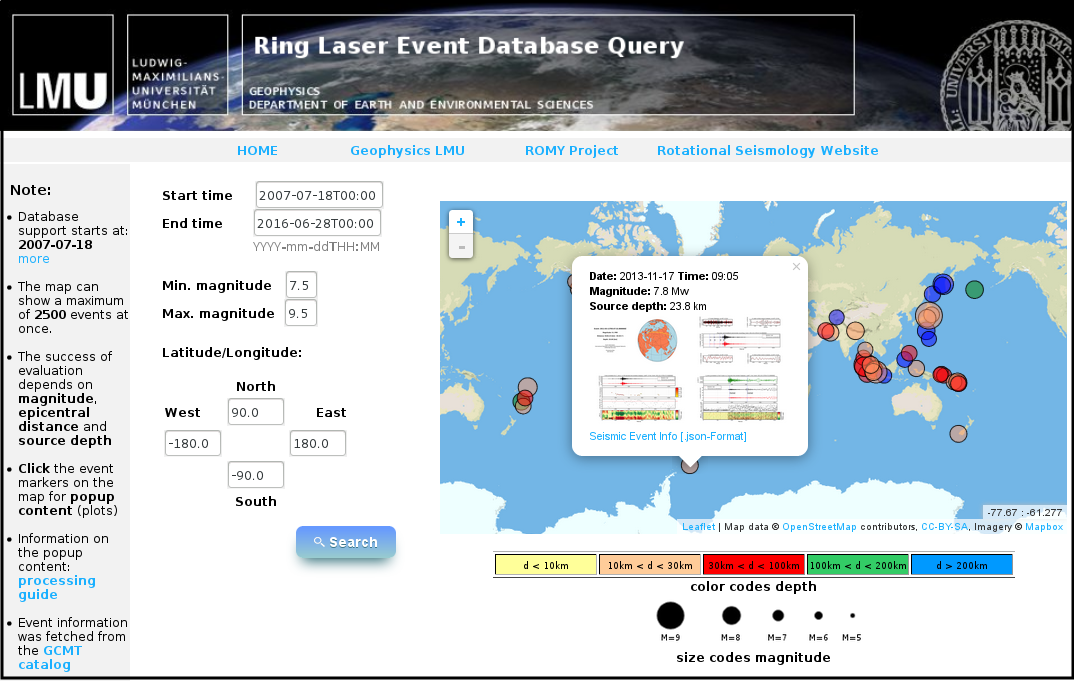
\includegraphics[width=\textwidth]{webpage_framed.png}
\caption{Web appearance of the ring laser event database.}
\label{fig:stretchmar}
\end{figure*}
The aim of creating this file is to publicly provide event characteristics that were processed consistently and can be used for further (statistical) analysis by the user.

In order to make the processing transparent and produced plots understandable, we include a downloadable 5-page processing guide (PDF) and Python-ObsPy based source code snippets. The
%
%%%%%%%%%%%%%%%%%%%%%%%%%%%%%%%%%%%%%%%%%%%%%%%%%%%%%%%%%%%%%%%%%%%%%%%%%%%%%%
%%%%%%%%% SECTION PROCESSING
%%%%%%%%%%%%%%%%%%%%%%%%%%%%%%%%%%%%%%%%%%%%%%%%%%%%%%%%%%%%%%%%%%%%%%%%%%%%%%
%
\section{Processing}
\label{sec:processing}
\subsection{Pre-processing}
The event database is automatically updated on a daily basis. It is fed by event quick solutions (xml-format) provided by the Global Centroid Moment Tensor (GCMT) catalog. This catalog contains global earthquake events featuring moment magnitudes $M_w$, usually larger than 4.5. The event-/data-download and processing is based on different ObsPy routines.
After fetching the event information (origin time, epicenter, depth, etc.), raw ring laser and collocated seismometer waveforms are downloaded via FDSN (“International Federation of Digital Seismograph Networks”) web service.
The pre-processing of the downloaded seismic data streams is determined by the source-receiver distance (cf. table 1). 
Firstly, the seismometer’s impulse response is remove,  a derivation of ground acceleration [nm/s²] from the measured ground velocity and scaling of the ring laser observation to [nrad/s] is performed. The traces are low-pass filtered to decrease the impact of high frequency body waves and the ambient “cultural noise”. Furthermore, for teleseismic events, we apply a bandstop-filter to erase the secondary microseism ($\approx$7s period) which is more prominent than the primary microseism \citep{Hadziioannou2012} and causes shifts in our backazimuth estimation especially for Mid- to South-Atlantic events.
%
\subsection{Love wave phase velocity estimation}
\begin{figure*}[!htp]
\centering
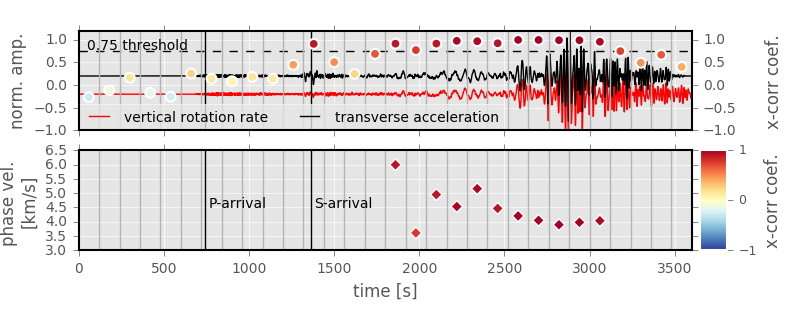
\includegraphics[width=\textwidth]{paper_plot1.png}
\caption{Visualization of the sliding window phase velocity estimation for the M9.0 Tohoku Oki earthquake, 2011. For each of the time windows, a cross-correlation is performed between vertical rotation rate and transverse acceleration (upper plot). We estimate phase velocities for windows associated with correlation coefficients larger than 0.75 and later than S-waves (lower plot).  }
\label{fig:stretchmar}
\end{figure*}
In order to derive Love wave phase velocities, the observed and pre-processed signals are compared analogous to \cite{Igel2005}: under the assumption of a transversely polarized plane wave, the vertical rotation rate and transverse acceleration are in phase and the amplitudes are related by: 
\begin{equation}
	\frac{a_t}{\dot{\Omega_z}} = -2c
\end{equation}
where c is the horizontal phase velocity \citep{McLeod1998, Pancha2000}. We therefor in a first step rotate (by the theoretical BAz) the horizontal acceleration components (North-East) in the source-receiver plane to Radial-Transverse to obtain a phase-match with the vertical rotation rate. The transverse acceleration and vertical rotation rate traces are then divided into sliding windows of equal size depending on the epicentral distance of the event (see table 1).
For each of these windows, a zero-lag normalized cross-correlation analysis is applied to $a_t$ and $\dot{\Omega_z}$ to check the coherence between the two waveforms (figure 2 [upper]). The resulting cross-correlation coefficient (CC) is used as a quality criterion (=threshold) for the determination of the phase velocities. For windows only featuring CC > 0.75, the horizontal phase velocity c is calculated by inserting peak values of $a_t$ and $\dot{\Omega_z}$ in the relation of equation 1 (figure 2 [lower]).
For “unfiltered” traces and high waveform coherence (=high quality signal) we will obtain an impression of the dispersive behaviour of Love waves right away by looking at the temporal evolution of the phase velocity. The dominant frequency of Love waves increases with time, so phase velocities decrease.

\subsection{Backazimuth Estimation}
\begin{figure*}[!htp]
\centering
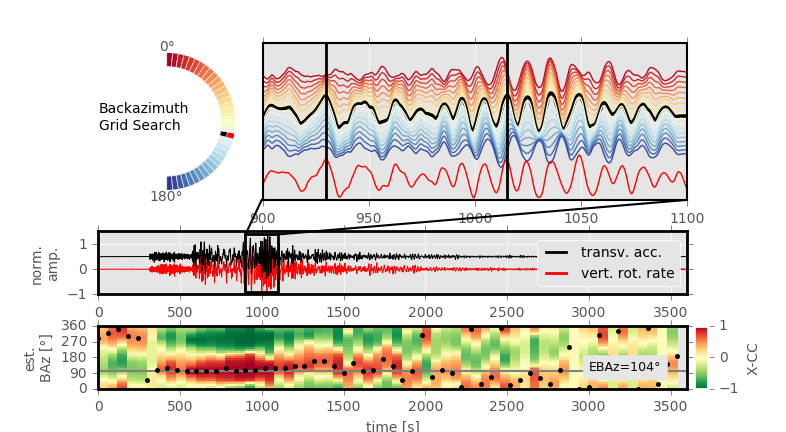
\includegraphics[width=\textwidth]{pp_Baz_paperready.png}
\caption{Illustration of the backazimuth estimation workflow. The grid search algorithm loops through all possible source directions in 1\textdegree -steps, cross-correlating the two traces of $a_t$ and $\dot{\Omega_z}$ for each time window (red = correlation; green = anti-correlation). The BAz-value related to maximum correlation is displayed as a black dot in the lowermost plot.}
\label{fig:stretchmar}
\end{figure*}
As in the phase velocity estimation and analogous to \cite{Igel2007} we investigate sliding windows throughout the signal to catch the evolution of the signal source direction, so again the traces are split into windows according to table 1. 
For each window, we estimate the direction of the signal in the two pre-processed traces employing a grid search optimization algorithm. The routine loops through all possible backazimuth directions (0° to 360°) in 1°- steps, for each step rotates the horizontal component acceleration (N-E) by the specified BAz-angle and then cross-correlates it with the vertical rotation rate. The CCs are maximal for a rotation from N-E to radial-transverse which is equivalent to rotating in the direction of the strongest signal source. In practice only widows reaching 90% correlation after rotation are considered in the estimation of the final BAz value, which is the average of the associated (CC>0.9) BAz results. 
Under the assumption of surface waves travelling on great circle paths, the conformity of theoretical and estimated BAz is a measure for the conformity of the two recorded measurands (rotation rate, transv. acc.) and thus for the resolution quality of the two instruments. (However, disparities between the two directions (theoretical, estimated) in combination with higher CCs on the estimated BAz side may indicate deviations of the actual Love wave path in the source-receiver plane. Thus, it might suggest heterogeneities/scatterers in the dimension of the wavelength along the direct wave path.) $\Rightarrow$ put into discussion?\\

\section{Discussion \& Conclusions}
Inclusion of other ring lasers (PFO, Christchurch, FFB, Gan Sasso?) in future\\
Actually just starting to use the deep underground ring laser GINGERino in the GranSasso!\\
Statistical evaluations: 
Magnitude scale based on rotational ground motions (Love waves)\\
(Local, one-station tomography)\\
Analysis of azimuthal effects
%%%%%%%%%%%%%%%%%%%%%%%%

\section*{Tables}
\begin{table}
	\begin{tabular}{l|ccccc}
	& \begin{tabular}{@{}c@{}}\textbf{distance}\\ \textbf{range}\end{tabular}& \begin{tabular}{@{}c@{}}\textbf{lowpass}\\ \textbf{cutoff}\end{tabular} & \begin{tabular}{@{}c@{}}\textbf{resampling}\\\textbf{decimation factor}\end{tabular} & \begin{tabular}{@{}c@{}}\textbf{cross-correlation}\\\textbf{window length}\end{tabular}& \begin{tabular}{@{}c@{}}\textbf{microseism}\\ \textbf{bandstop}\end{tabular}\\
	\hline
	\textbf{close} & 0\textdegree$\le d \le$3\textdegree & 4 Hz & 2 & 3 s & - \\
	\hline
	\textbf{local} & 3\textdegree$\le d \le$10\textdegree & 2 Hz & 2 & 5 s & - \\
	\hline
	\textbf{tele} & $d >$10\textdegree & 1 Hz & 4 & 120 s & 5 s - 12 s \\  
	
	\end{tabular}
	\label{table1}
	\caption{Pre-processing parameter table for different source-receiver distances.}
\end{table}

\section*{ACKNOWLEDGMENTS}
We would like to thank ...



\label{Bibliography}
%\begin{thebibliography}{99}
\bibliography{Bibliography_ROMY.bib}
%
%\newcommand{\enquote}[1]{``#1''}
%\providecommand{\bibinfo}[2]{#2}
%\providecommand{\noopsort}[1]{}
%\providecommand{\switchargs}[2]{#2#1}
%
%\bibitem{cunha2006}
%\bibinfo{author}{{\'A}.~Cunha} and \bibinfo{author}{E.~Caetano},
%  \enquote{\bibinfo{title}{Experimental modal analysis of civil engineering
%  structures}}, \bibinfo{journal}{Sound and Vibration}
%  \textbf{\bibinfo{volume}{40}}, \bibinfo{pages}{12--20}
%  (\bibinfo{year}{2006}).
%
%\bibitem{Magalhaes2011}
%\bibinfo{author}{F.~Magalh{\~a}es}, \bibinfo{author}{A.~Cunha}, and
%  \bibinfo{author}{E.~Caetano}, \enquote{\bibinfo{title}{Vibration based
%  structural health monitoring of an arch bridge: From automated {OMA} to
%  damage detection}}, \bibinfo{journal}{Mech Syst Signal Pr}
%  \textbf{\bibinfo{volume}{28}}, \bibinfo{pages}{212 -- 228}
%  (\bibinfo{year}{2012}).
%
%\bibitem{Rainieri2010}
%\bibinfo{author}{C.~Rainieri} and \bibinfo{author}{G.~Fabbrocino},
%  \enquote{\bibinfo{title}{Automated output-only dynamic identification of
%  civil engineering structures}}, \bibinfo{journal}{Mech Syst Signal Pr}
%  \textbf{\bibinfo{volume}{24}}, \bibinfo{pages}{678 -- 695}
%  (\bibinfo{year}{2010}).
%
%\bibitem{Ubertini2012}
%\bibinfo{author}{F.~Ubertini}, \bibinfo{author}{A.~L. Materazzi},
%  \bibinfo{author}{C.~Gentile}, and \bibinfo{author}{F.~Pelliccia},
%  \enquote{\bibinfo{title}{Automatic identification of modal parameters:
%  application to a reinforced concrete arch bridge}}, \bibinfo{journal}{Proc.
%  EACS}  (\bibinfo{year}{2012}).
%
%\bibitem{Planes2013}
%\bibinfo{author}{T.~Plan{\`e}s} and \bibinfo{author}{E.~Larose},
%  \enquote{\bibinfo{title}{A review of ultrasonic {C}oda {W}ave
%  {I}nterferometry in concrete}}, \bibinfo{journal}{Cement and Concrete
%  Research} \textbf{\bibinfo{volume}{53}}, \bibinfo{pages}{248 -- 255}
%  (\bibinfo{year}{2013}).
%
%\bibitem{Larose2006}
%\bibinfo{author}{E.~Larose}, \bibinfo{author}{J.~de~Rosny},
%  \bibinfo{author}{L.~Margerin}, \bibinfo{author}{D.~Anache},
%  \bibinfo{author}{P.~Gouedard}, \bibinfo{author}{M.~Campillo}, and
%  \bibinfo{author}{B.~van Tiggelen}, \enquote{\bibinfo{title}{Observation of multiple scattering of kHz vibrations in a concrete structure and application to monitoring weak changes}}, \bibinfo{journal}{Phys. Rev. E}
%  \textbf{\bibinfo{volume}{73}}, \bibinfo{pages}{016609--016616}
%  (\bibinfo{year}{2006}).
%
%\bibitem{Niederleithinger2013}
%\bibinfo{author}{E.~Niederleithinger} and \bibinfo{author}{C.~Wunderlich},
%  \enquote{\bibinfo{title}{Influence of small temperature variations on the ultrasonic velocity in concrete}}, \bibinfo{journal}{AIP Conference
%  Proceedings} \textbf{\bibinfo{volume}{1511}}, \bibinfo{pages}{390--397}
%  (\bibinfo{year}{2013}).
%
%\bibitem{Gret2006}
%\bibinfo{author}{A.~Gr{\^e}t}, \bibinfo{author}{R.~Snieder}, and
%  \bibinfo{author}{J.~Scales}, \enquote{\bibinfo{title}{Time-lapse monitoring of rock properties with coda wave interferometry}}, \bibinfo{journal}{J.  Geophys. Res. Solid Earth} \textbf{\bibinfo{volume}{111}},
%  \bibinfo{pages}{1978--2012} (\bibinfo{year}{2006}).
%  
%\bibitem{Staehler2011}
%\bibinfo{author}{S.~C. St{\"a}hler}, \bibinfo{author}{C.~Sens-Sch{\"o}nfelder}, and
%  \bibinfo{author}{E.~Niederleithinger}, \enquote{\bibinfo{title}{Monitoring
%  stress changes in a concrete bridge with coda wave interferometry}},
%  \bibinfo{journal}{J. Acoust. Soc. Am.} \textbf{\bibinfo{volume}{129}},
%  \bibinfo{pages}{1945--1952} (\bibinfo{year}{2011}).
%
%\bibitem{Lobkis2001}
%\bibinfo{author}{O.~Lobkis} and \bibinfo{author}{R.~L. Weaver},
%  \enquote{\bibinfo{title}{{On the emergence of the Green's function in the correlations of a diffuse field}}}, \bibinfo{journal}{J. Acoust. Soc. Am.} \textbf{\bibinfo{volume}{110}}, \bibinfo{pages}{3011--3017}
%  (\bibinfo{year}{2001}).
%
%\bibitem{Shapiro2005}
%\bibinfo{author}{N.~M. Shapiro}, \bibinfo{author}{M.~Campillo},
%  \bibinfo{author}{L.~Stehly}, and \bibinfo{author}{M.~H. Ritzwoller},
%  \enquote{\bibinfo{title}{High-resolution surface-wave tomography from ambient
%  seismic noise}}, \bibinfo{journal}{Science} \textbf{\bibinfo{volume}{307}},
%  \bibinfo{pages}{1615--1618} (\bibinfo{year}{2005}).
%
%\bibitem{SensS2006}
%\bibinfo{author}{C.~Sens-Sch{\"o}nfelder} and \bibinfo{author}{U.~Wegler},
%  \enquote{\bibinfo{title}{Passive image interferometry and seasonal variations
%  of seismic velocities at {M}erapi volcano, {I}ndonesia}},
%  \bibinfo{journal}{Geophys. Res. Lett.} \textbf{\bibinfo{volume}{33}},
%  \bibinfo{pages}{L21302} (\bibinfo{year}{2006}).
%
%\bibitem{Wegler2007}
%\bibinfo{author}{U.~Wegler} and \bibinfo{author}{C.~Sens-Sch{\"o}nfelder},
%  \enquote{\bibinfo{title}{Fault zone monitoring with {P}assive {I}mage
%  {I}nterferometry}}, \bibinfo{journal}{Geophys. J. Int.}
%  \textbf{\bibinfo{volume}{168}}, \bibinfo{pages}{1029--1033}
%  (\bibinfo{year}{2007}).
%
%\bibitem{brenguier2008b}
%\bibinfo{author}{F.~Brenguier}, \bibinfo{author}{N.~M. Shapiro},
%  \bibinfo{author}{M.~Campillo}, \bibinfo{author}{V.~Ferrazzini},
%  \bibinfo{author}{Z.~Duputel}, \bibinfo{author}{O.~Coutant}, and
%  \bibinfo{author}{A.~Nercessian}, \enquote{\bibinfo{title}{{Towards
%  forecasting volcanic eruptions using seismic noise}}},
%  \bibinfo{journal}{Nature Geoscience} \textbf{\bibinfo{volume}{1}},
%  \bibinfo{pages}{126--130} (\bibinfo{year}{2008}).
%
%\bibitem{Snieder2002}
%\bibinfo{author}{R.~Snieder}, \bibinfo{author}{A.~Gr{\^e}t},
%  \bibinfo{author}{H.~Douma}, and \bibinfo{author}{J.~Scales},
%  \enquote{\bibinfo{title}{Coda wave interferometry for estimating nonlinear
%  behavior in seismic velocity}}, \bibinfo{journal}{Science}
%  \textbf{\bibinfo{volume}{295}}, \bibinfo{pages}{2253--2255}
%  (\bibinfo{year}{2002}).
%
%\bibitem{Poupinet1984}
%\bibinfo{author}{G.~Poupinet}, \bibinfo{author}{W.~L. Ellsworth}, and
%  \bibinfo{author}{J.~Frechet}, \enquote{\bibinfo{title}{Monitoring velocity
%  variations in the crust using earthquake doublets: An application to the
%  {C}alaveras {F}ault, {C}alifornia}}, \bibinfo{journal}{J. Geophys. Res. Solid
%  Earth} \textbf{\bibinfo{volume}{89}}, \bibinfo{pages}{5719--5731}
%  (\bibinfo{year}{1984}).
%
%\bibitem{Rosetto2011}
%\bibinfo{author}{V.~Rossetto}, \bibinfo{author}{L.~Margerin},
%  \bibinfo{author}{T.~Plan{\`e}s}, and \bibinfo{author}{E.~Larose},
%  \enquote{\bibinfo{title}{Locating a weak change using diffuse waves:
%  Theoretical approach and inversion procedure}}, \bibinfo{journal}{Journal of
%  Applied Physics} \textbf{\bibinfo{volume}{109}}, \bibinfo{pages}{--}
%  (\bibinfo{year}{2011}).
%
%\bibitem{Planes2014}
%\bibinfo{author}{T.~Plan{\`e}s}, \bibinfo{author}{E.~Larose},
%  \bibinfo{author}{L.~Margerin}, \bibinfo{author}{V.~Rossetto}, and
%  \bibinfo{author}{C.~Sens-Sch{\"o}nfelder},
%  \enquote{\bibinfo{title}{Decorrelation and phase-shift of coda waves induced
%  by local changes: multiple scattering approach and numerical validation}},
%  \bibinfo{journal}{Waves in Random and Complex Media}
%  \textbf{\bibinfo{volume}{24}}, \bibinfo{pages}{99--125}
%  (\bibinfo{year}{2014}).
%
%\bibitem{Lobkis2003}
%\bibinfo{author}{O.~I. Lobkis} and \bibinfo{author}{R.~L. Weaver},
%  \enquote{\bibinfo{title}{Coda-wave interferometry in finite solids: Recovery
%  of P-to-S conversion rates in an elastodynamic billiard}},
%  \bibinfo{journal}{Phys. Rev. Lett.} \textbf{\bibinfo{volume}{90}},
%  \bibinfo{pages}{254302--254306} (\bibinfo{year}{2003}).
%
%\bibitem{Shapiro2004}
%\bibinfo{author}{N.~M. Shapiro} and \bibinfo{author}{M.~Campillo},
%  \enquote{\bibinfo{title}{Emergence of broadband {R}ayleigh waves from
%  correlations of the ambient seismic noise}}, \bibinfo{journal}{Geophys. Res.
%  Lett.} \textbf{\bibinfo{volume}{31}}, \bibinfo{pages}{L07614}
%  (\bibinfo{year}{2004}).
%
%\bibitem{Hadziioannou2011}
%\bibinfo{author}{C.~Hadziioannou}, \bibinfo{author}{E.~Larose},
%  \bibinfo{author}{A.~Baig}, \bibinfo{author}{P.~Roux}, and
%  \bibinfo{author}{M.~Campillo}, \enquote{\bibinfo{title}{Improving temporal
%  resolution in ambient noise monitoring of seismic wave speed}},
%  \bibinfo{journal}{J. Geophys. Res. Solid Earth}
%  \textbf{\bibinfo{volume}{116}}, \bibinfo{pages}{1978--2012}
%  (\bibinfo{year}{2011}).
%
%\bibitem{Obspy2010}
%\bibinfo{author}{M.~Beyreuther}, \bibinfo{author}{R.~Barsch},
%  \bibinfo{author}{L.~Krischer}, \bibinfo{author}{T.~Megies},
%  \bibinfo{author}{Y.~Behr}, and \bibinfo{author}{J.~Wassermann},
%  \enquote{\bibinfo{title}{Obspy: A {P}ython toolbox for seismology}},
%  \bibinfo{journal}{Seis. Res. Lett.} \textbf{\bibinfo{volume}{81}},
%  \bibinfo{pages}{530--533} (\bibinfo{year}{2010}).
%
%\bibitem{NumPy}
%\bibinfo{author}{P.~F. Dubois}, \bibinfo{author}{K.~Hinsen}, and
%  \bibinfo{author}{J.~Hugunin}, \enquote{\bibinfo{title}{Numerical {P}ython}},
%  \bibinfo{journal}{Computers in Physics} \textbf{\bibinfo{volume}{10}}
%  (\bibinfo{year}{1996}).
%
%\bibitem{NumPy2}
%\bibinfo{author}{D.~Ascher}, \bibinfo{author}{P.~Dubois},
%  \bibinfo{author}{K.~Hinsen}, \bibinfo{author}{J.~Hugunin},
%  \bibinfo{author}{T.~Oliphant},
%  \enquote{\bibinfo{title}{An open source project: Numerical {P}ython}}, \bibinfo{journal}{Technical Report UCRL-MA-128569, Lawrence Livermore National Laboratory}  (\bibinfo{year}{2001}).
%
%\bibitem{Cupillard2011}
%\bibinfo{author}{P.~Cupillard}, \bibinfo{author}{L.~Stehly}, and
%  \bibinfo{author}{B.~Romanowicz}, \enquote{\bibinfo{title}{The one-bit noise
%  correlation: a theory based on the concepts of coherent and incoherent
%  noise}}, \bibinfo{journal}{Geophys. J. Int.} \textbf{\bibinfo{volume}{184}},
%  \bibinfo{pages}{1397--1414} (\bibinfo{year}{2011}).
%
%\bibitem{Keller1992}
%\bibinfo{author}{T.~Keller} and \bibinfo{author}{C.~Menn},
%  \enquote{\bibinfo{title}{Dauerhaftigkeit von {S}tahlbetontragwerken:
%  {T}ransportmechanismen -- {A}uswirkungen von {R}issen} (Durability of reinforced concrete structures: Transportmechanis-
%men -- effects of cracks)},
%  \bibinfo{type}{Technical Report} (\bibinfo{year}{1992}).
%
%\bibitem{BS1881}
%\bibinfo{author}{British-Standard-Institution}, \emph{\bibinfo{title}{BS 1881,
%  Part 203, Recommendations for Measurement of Velocity of Ultrasonic Pulses in
%  Concrete}}, \bibinfo{address}{London} (\bibinfo{year}{1986}).
%
%\bibitem{Peeters2001}
%\bibinfo{author}{B.~Peeters} and \bibinfo{author}{G.~De~Roeck},
%  \enquote{\bibinfo{title}{One-year monitoring of the {Z24}-{B}ridge:
%  environmental effects versus damage events}}, \bibinfo{journal}{Earthquake
%  Engineering \& Structural Dynamics} \textbf{\bibinfo{volume}{30}},
%  \bibinfo{pages}{149--171} (\bibinfo{year}{2001}).
%
%\bibitem{Celine2009}
%\bibinfo{author}{C.~Hadziioannou}, \bibinfo{author}{E.~Larose},
%  \bibinfo{author}{O.~Coutant}, \bibinfo{author}{P.~Roux}, and
%  \bibinfo{author}{M.~Campillo}, \enquote{\bibinfo{title}{Stability of
%  monitoring weak changes in multiply scattering media with ambient noise
%  correlation: Laboratory experiments}}, \bibinfo{journal}{J. Acoust. Soc. Am.}
%  \textbf{\bibinfo{volume}{125}}, \bibinfo{pages}{3688--3695}
%  (\bibinfo{year}{2009}).

%\end{thebibliography}


\newpage

\noindent
{\large \textbf{FIGURE CAPTIONS}}

\noindent
Figure 1: Real data example for extreme temperature cases; 'cold'(blue): cross-correlation of 1 hour of noise recorded at two receivers at a temperature of -23\textdegree{C}, 'hot'(red): same for temperature of +13\textdegree{C}, black dashed line: reference signal consisting of the average of all cross-correlations from the total recording time. The signal recorded on a cold day is clearly compressed compared to the reference, the signal corresponding to a hot day is stretched. The displacement amplitudes are normalized.

\noindent
Figure 2: (a) Lateral view on the 229~m long Steinachtal bridge (scheme) looking north-ward. Bars indicate the positions of geophones in the box girder. (b) Cross-section of the box girder with geophone position indicated by a triangle. (c) The photo shows the bridge in construction state, viewed from below. (d) Attachment of a geophone to the bridge. The instrument was screwed on a footplate slab, which was then cemented onto the bridge. It was not possible to drill holes into the bridge itself.

\noindent
Figure 3: (a) Waveform recorded for a car passing over the bridge and (b) spectrogram for this event. Characteristic features of this signal are two clear onsets (corresponding to the vehicle passing the expansion gap at either end of the bridge) and distinct reverberations. The amplitudes suggest that the car passed the more distant extension gap first, i.e. that it was traveling east-ward (compare fig. \ref{fig:SteinachtalBridge}a). The time difference of roughly 10 seconds between the crossings of the two gaps correspond to a car velocity of roughly 80 km/h, which is indeed the local speed limit.


\noindent   
\noindent   

\end{document}
%
% ****** End of file jasatmpl.tex ******
